\documentclass{beamer}
\mode<presentation> {

\usepackage{color}
\definecolor{bottomcolour}{rgb}{0.21,0.11,0.21}
\definecolor{middlecolour}{rgb}{0.21,0.11,0.21}
\setbeamercolor{structure}{fg=white}
\setbeamertemplate{frametitle}[default]%[center]
\setbeamercolor{normal text}{bg=black, fg=white}
\setbeamertemplate{background canvas}[vertical shading]
[bottom=bottomcolour, middle=middlecolour, top=black]
\setbeamertemplate{items}[circle]
\setbeamertemplate{navigation symbols}{} %no nav symbols
\setbeamercolor{block title}{use=structure,fg=white,bg=structure.fg!50!red!50!blue!100!green}
\setbeamercolor{block body}{parent=normal text,use=block title,bg=block title.bg!5!white!10!bg,fg=white}
\setbeamertemplate{navigation symbols}{}
}
\usepackage{graphicx} 
\usepackage{booktabs} 
\usepackage[utf8]{inputenc}  
\usepackage[T1]{fontenc}  
\usepackage{geometry}     
\usepackage[francais]{babel} 
\usepackage{eurosym}
\usepackage{verbatim}
\usepackage{ragged2e}
\justifying
%%%%%%%%%%%%%%%%%%%%%%%%%%%%%%%%%%%%%%%%%%%%%%%%%%%%%%%%%%%%%%%%
%% ccBeamer 0.1, 2007-07-02                                   %%
%% Written by Sebastian Pipping <webmaster@hartwork.org>      %%
%% ---------------------------------------------------------- %%
%% Licensed under Creative Commons Attribution-ShareAlike 3.0 %%
%% http://creativecommons.org/licenses/by-sa/3.0/             %%
%%%%%%%%%%%%%%%%%%%%%%%%%%%%%%%%%%%%%%%%%%%%%%%%%%%%%%%%%%%%%%%%


%% Images
\newcommand{\CcImageBy}[1]{%
	
\includegraphics[scale=#1]{creative_commons/cc_by_30.pdf}%
}
\newcommand{\CcImageCc}[1]{%
	
\includegraphics[scale=#1]{creative_commons/cc_cc_30.pdf}%
}
\newcommand{\CcImageDevNations}[1]{%
	
\includegraphics[scale=#1]{creative_commons/cc_dev_nations_30.pdf}%
}
\newcommand{\CcImageNc}[1]{%
	
\includegraphics[scale=#1]{creative_commons/cc_nc_30.pdf}%
}
\newcommand{\CcImageNd}[1]{%
	
\includegraphics[scale=#1]{creative_commons/cc_nd_30.pdf}%
}
\newcommand{\CcImagePd}[1]{%
	
\includegraphics[scale=#1]{creative_commons/cc_pd_30.pdf}%
}
\newcommand{\CcImageSa}[1]{%
	
\includegraphics[scale=#1]{creative_commons/cc_sa_30.pdf}%
}
\newcommand{\CcImageSampling}[1]{%
	
\includegraphics[scale=#1]{creative_commons/cc_sampling_30.pdf}%
}
\newcommand{\CcImageSamplingPlus}[1]{%
	
\includegraphics[scale=#1]{creative_commons/cc_sampling_plus_30.pdf}%
}


%% Groups
\newcommand{\CcGroupBy}[1]{% zoom
	\CcImageBy{#1}%
}
\newcommand{\CcGroupByNc}[2]{% zoom, gap
	\CcImageBy{#1}\hspace*{#2}\CcImageNc{#1}%
}
\newcommand{\CcGroupByNcNd}[2]{% zoom, gap
	\CcImageBy{#1}\hspace*{#2}\CcImageNc{#1}\hspace*{#2}\CcImageNd{#1}%
}
\newcommand{\CcGroupByNcSa}[2]{% zoom, gap
	\CcImageBy{#1}\hspace*{#2}\CcImageNc{#1}\hspace*{#2}\CcImageSa{#1}%
}
\newcommand{\CcGroupByNd}[2]{% zoom, gap
	\CcImageBy{#1}\hspace*{#2}\CcImageNd{#1}%
}
\newcommand{\CcGroupBySa}[2]{% zoom, gap
	\CcImageBy{#1}\hspace*{#2}\CcImageSa{#1}%
}
\newcommand{\CcGroupDevNations}[1]{% zoom
	\CcImageDevNations{#1}%
}
\newcommand{\CcGroupNcSampling}[2]{% zoom, gap
	\CcImageNc{#1}\hspace*{#2}\CcImageSampling{#1}%
}
\newcommand{\CcGroupPd}[1]{% zoom
	\CcImagePd{#1}%
}
\newcommand{\CcGroupSampling}[1]{% zoom
	\CcImageSampling{#1}%
}
\newcommand{\CcGroupSamplingPlus}[1]{% zoom
	\CcImageSamplingPlus{#1}%
}


%% Text
\newcommand{\CcLongnameBy}{Attribution}
\newcommand{\CcLongnameByNc}{Attribution-NonCommercial}
\newcommand{\CcLongnameByNcNd}{Attribution-NoDerivs}
\newcommand{\CcLongnameByNcSa}{Attribution-NonCommercial-ShareAlike}
\newcommand{\CcLongnameByNd}{Attribution-NoDerivs}
\newcommand{\CcLongnameBySa}{Attribution-ShareAlike}

\newcommand{\CcNote}[1]{% longname
	This work is licensed under the \textit{Creative Commons #1 3.0 License}.%
}

\title[Tor et le Tor Browser Bundle]{Le réseau Tor} 
\author{Genma}
\date{Ubuntu Party - 30-31 mai 2015}
\begin{document}
\begin{frame}
	\titlepage
	\begin{center}
		
\includegraphics[scale=0.2]{./images/logo_tor.jpg}
		\\		
		\CcGroupByNcSa{0.83}{0.95ex}\\[2.5ex]
		{\tiny\CcNote{\CcLongnameByNcSa}}
		\vspace*{-2.5ex}
	\end{center}
\end{frame}

\begin{frame}
\frametitle{
\includegraphics[scale=0.4]{./images/Genma.jpg} \ \ \  A propos de moi  }
\begin{columns}[c] 

\column{.55\textwidth} 
\textbf{Où me trouver sur Internet?}
\begin{itemize}
\item Le Blog de Genma : http://genma.free.fr
\item Twitter : http://twitter.com/genma
\end{itemize}
\textbf{Mes projets-contributions}
\\ Plein de choses dont:
\begin{itemize}
\item Promotion de Tor
\item A.I.\up{2} Apprenons l'Informatique, Apprenons Internet
\end{itemize}

\column{.5\textwidth} 
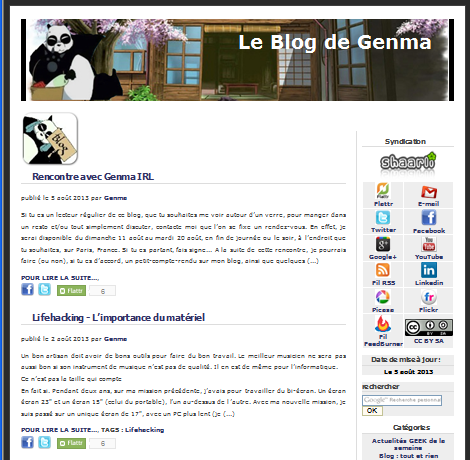
\includegraphics[width=5cm,height=5cm]{./images/blog.png} 
\end{columns}
\end{frame}

%----------------------------------------------------------------------------------------
\begin{frame}
\frametitle{Remerciements}
Je remercie l'association NosOignons.net, qui propose des nœuds de sortie Tor financés par la communauté.
\url{https://nos-oignons.net}
\\~\\

\includegraphics[scale=0.4]{./images/NosOignons.jpg}
\end{frame}
%----------------------------------------------------------------------------------------
\begin{frame}
\begin{center}
\Huge{Introduction}
\\~\\ 
\includegraphics[scale=0.4]{./images/logo_tor.jpg}
\end{center}
\end{frame}
%----------------------------------------------------------------------------------------
\begin{frame}
\frametitle{Présentation du réseau TOR}
Tor est un logiciel libre,
\begin{itemize}
\item grâce auquel existe le réseau d'anonymisation Tor
\item  soutenu par l'organisation The Tor Project.
\end{itemize}
$\Rightarrow$ Techniquement, Tor nous permet de se connecter à des machines sur Internet via des relais. 
\\$\Rightarrow$ Et cela de façon à ce qu'elles ne puissent pas identifier notre connexion (et donc de nous localiser).
\end{frame}
%----------------------------------------------------------------------------------------
\begin{frame}
\begin{center}
\Huge{A quoi sert TOR?}
\\~\\ 
\includegraphics[scale=0.4]{./images/logo_tor.jpg}
\end{center}
\end{frame}
%----------------------------------------------------------------------------------------
\begin{frame}
\frametitle{A quoi sert TOR?}
Concrêtement, ça sert pour :
\begin{itemize}
\justifying{
\item  échapper au fichage publicitaire,
\item  publier des informations sous un pseudonyme,
\item  accéder à des informations en laissant moins de traces,
\item  déjouer des dispositifs de filtrage (dans sa fac, en Chine ou en Iran…),
\item  communiquer en déjouant des dispositifs de surveillances,
\item  tester son pare-feu,
\item  … et sûrement encore d'autres choses.
}
\end{itemize}
\justifying{
$\Rightarrow$ Tor dispose également d'un système de « services cachés » qui permet de fournir un service en cachant l'emplacement du serveur.
}
\end{frame}
%----------------------------------------------------------------------------------------
\begin{frame}
\begin{center}
\Huge{Comment fonctionne Tor ? }
\\~\\ 
\includegraphics[scale=0.4]{./images/logo_tor.jpg}
\end{center}
\end{frame}
%----------------------------------------------------------------------------------------
\begin{frame}
\frametitle{Comment fonctionne Tor ?}
\begin{center}
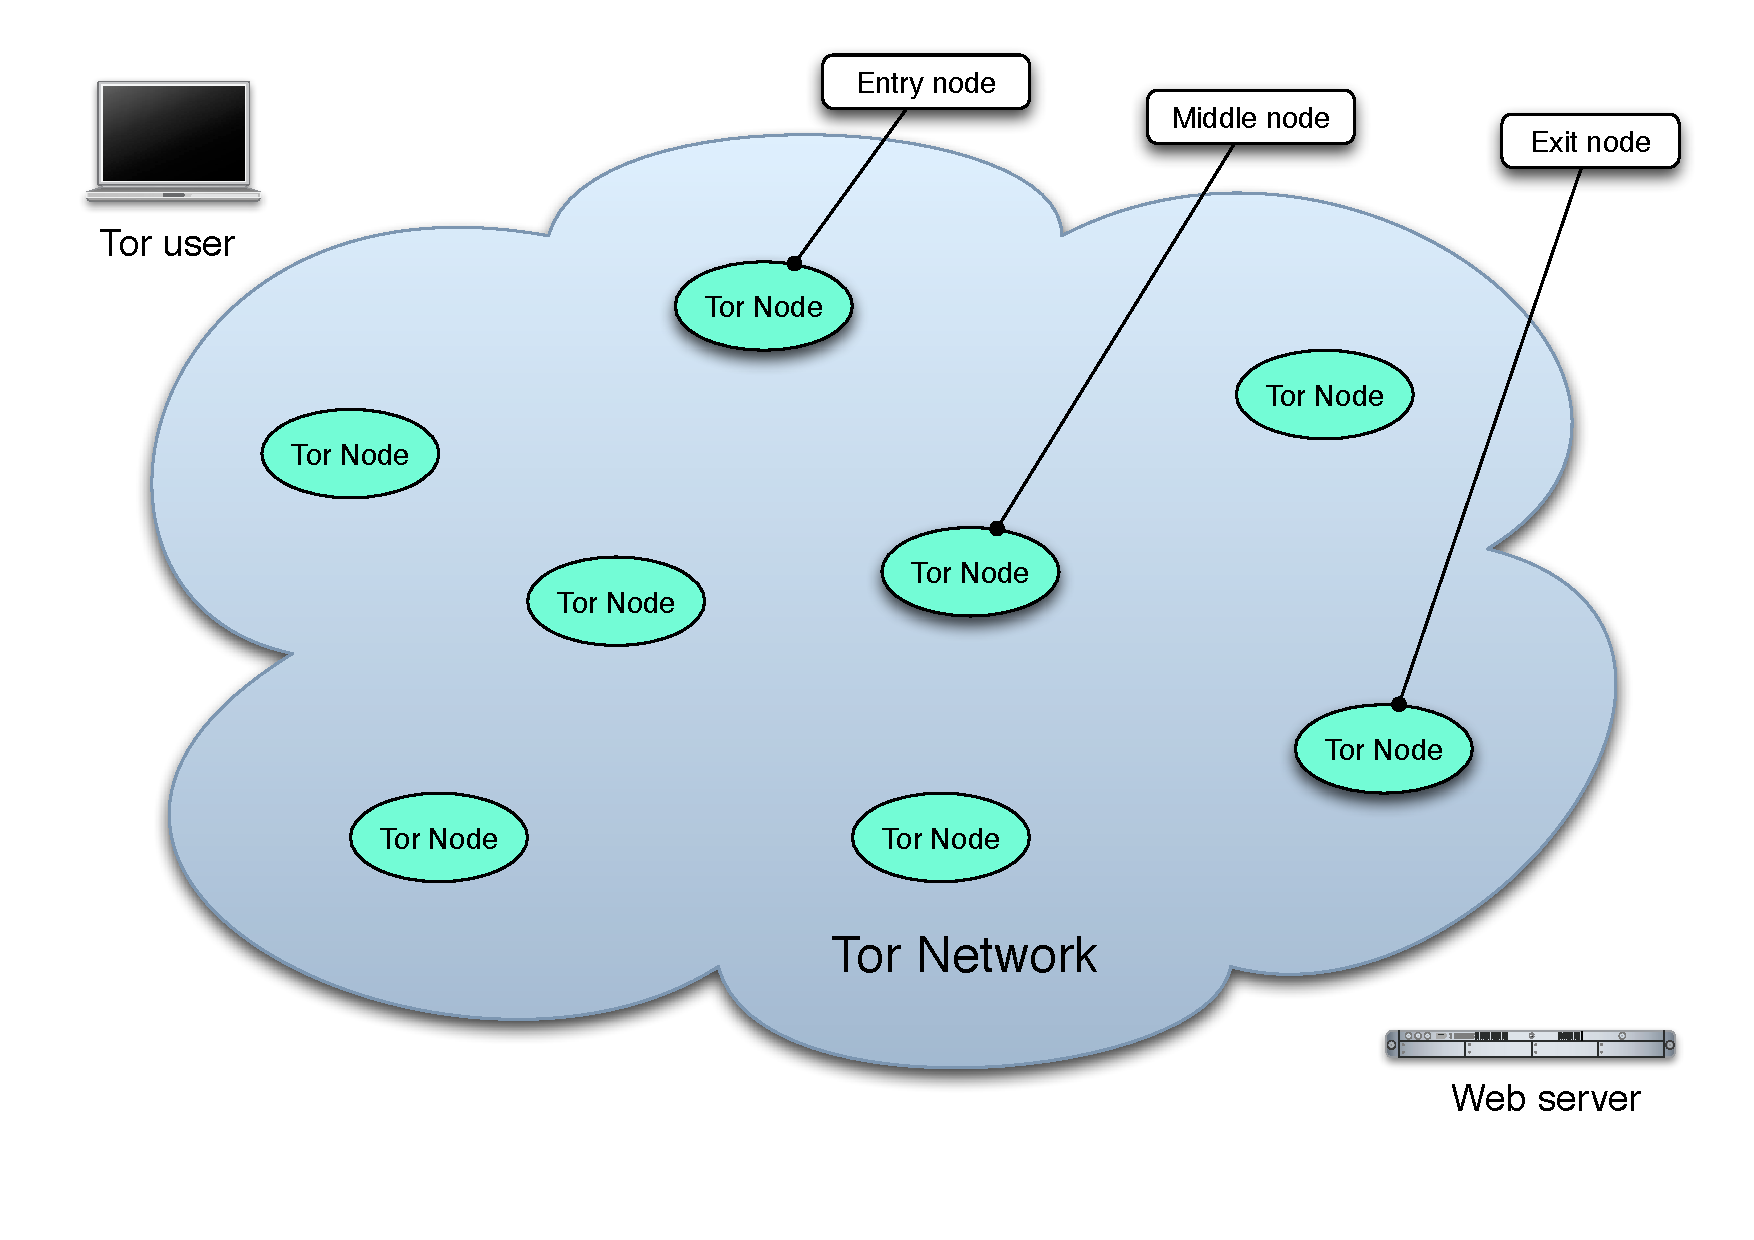
\includegraphics[keepaspectratio,width=\textwidth, height=.8\textheight]{images/tor-safe-selection}
\end{center}
\end{frame}
%----------------------------------------------------------------------------------------
\begin{frame}
\frametitle{Comment fonctionne Tor ?}
\begin{center}
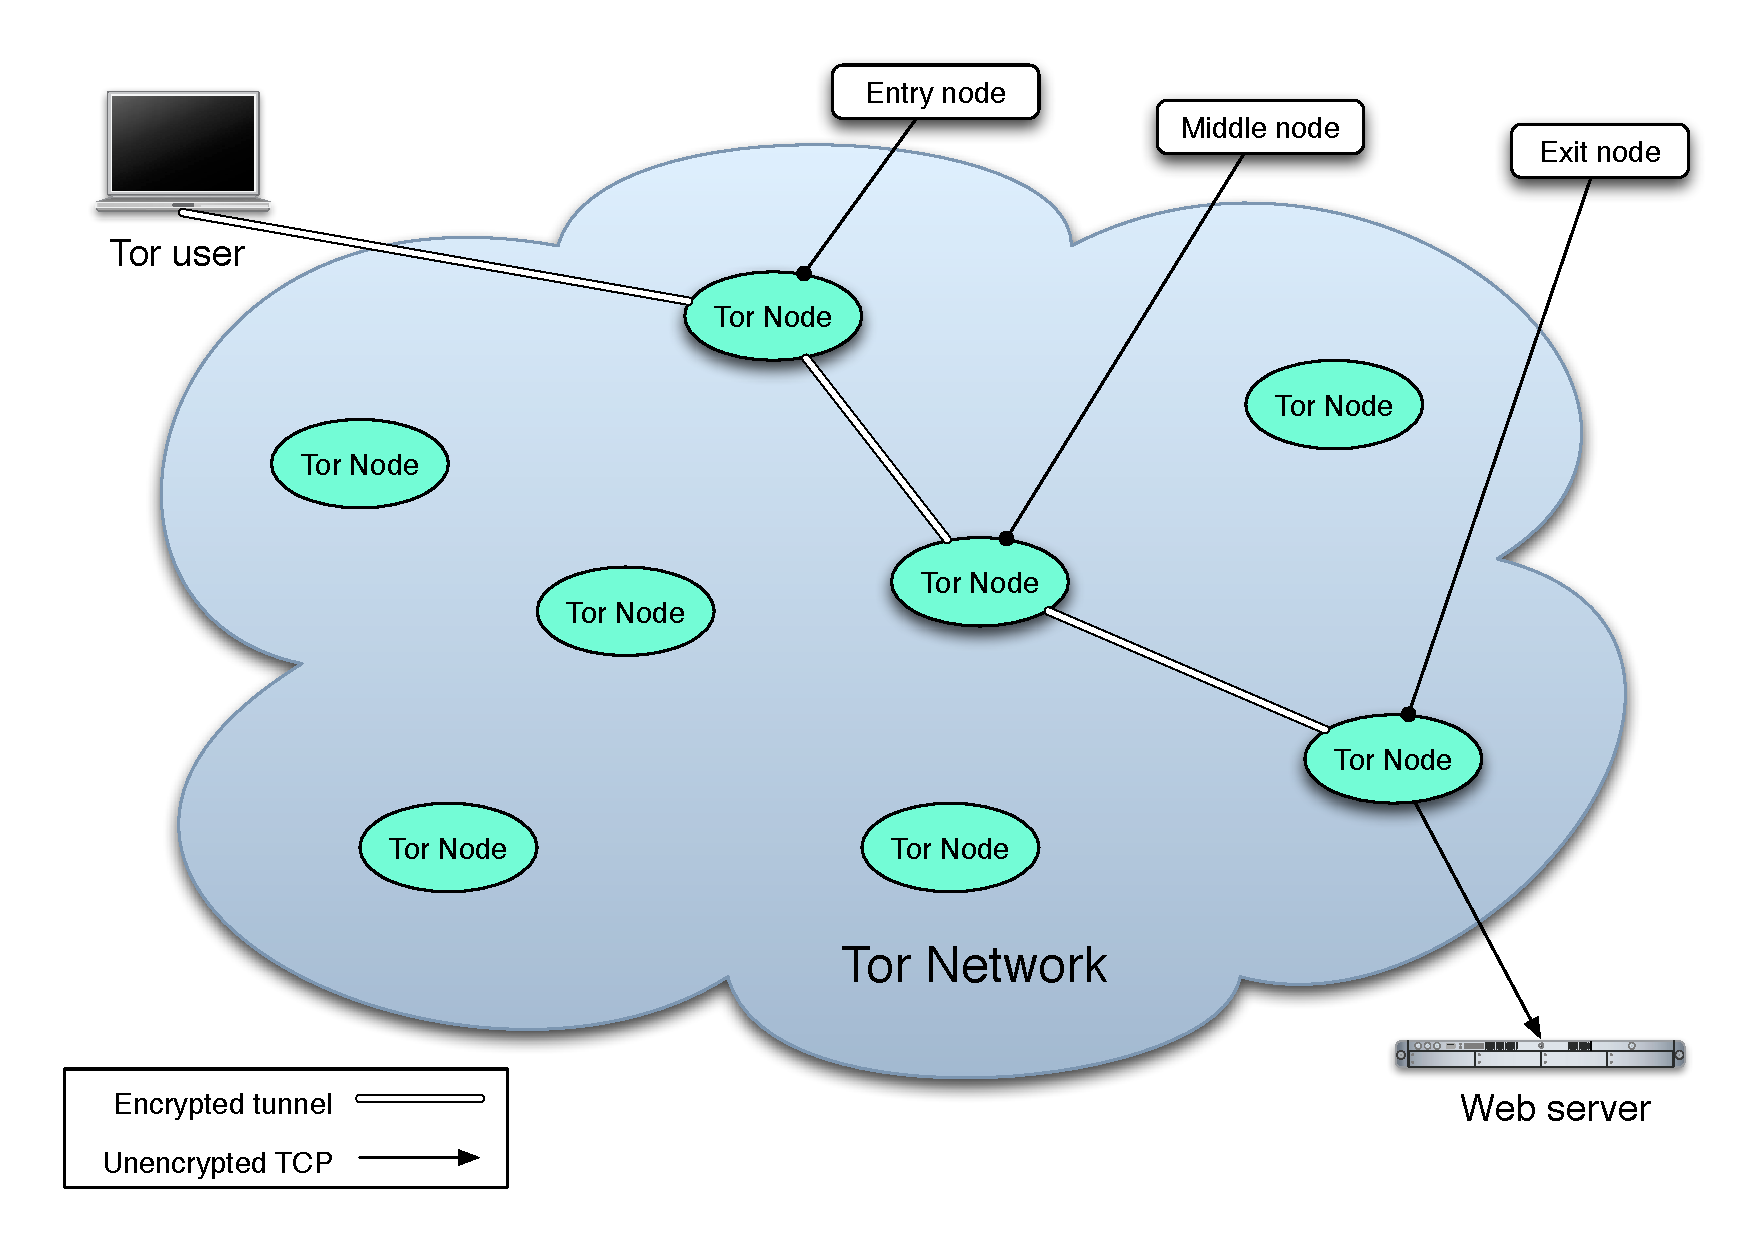
\includegraphics[keepaspectratio,width=\textwidth, height=.8\textheight]{images/tor-safe-path}
\end{center}
\end{frame}
%----------------------------------------------------------------------------------------
\begin{frame}
\frametitle{Comment fonctionne Tor ?}
\begin{center}
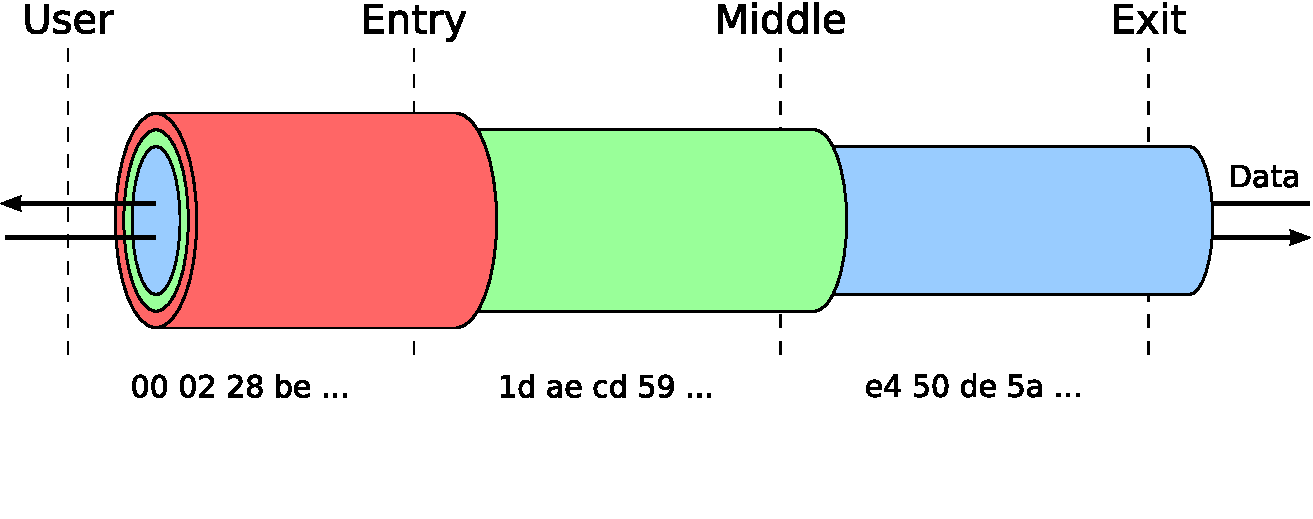
\includegraphics[keepaspectratio,width=\textwidth, height=.8\textheight]{images/tor-keys1}
\end{center}
\end{frame}
%----------------------------------------------------------------------------------------
\begin{frame}
\frametitle{Comment fonctionne Tor ?}

\begin{itemize}
\justifying{
\item Tor fait un routage en oignion avec des couches de chiffrement empilées.
\item Il y a une première clé de chiffrement vers le nœud d'entrée, une second clé vers le nœud du milieu et
une dernière pour le nœud de sortie.
}
\end{itemize}
\justifying{
$\Rightarrow$ Tor ne chiffre pas après le noeud de sortie.
\\
$\Rightarrow$ Il faut utiliser une connexion httpS.
}
\end{frame}
%----------------------------------------------------------------------------------------
\begin{frame}
\begin{center}
\Huge{Tor hidden service \\ les services cachés de TOR}
\\~\\ 
\includegraphics[scale=0.4]{./images/logo_tor.jpg}
\end{center}
\end{frame}
%----------------------------------------------------------------------------------------
\begin{frame}
\frametitle{Tor hidden service - les services cachés de TOR}
\justifying{
Tor permet aux clients et aux relais d’offrir des services cachés.Il est possible d'offrir un serveur web, un serveur SSH, etc, sans révéler son adresse IP aux utilisateurs.
}
\begin{itemize}
\justifying{
\item Tous ces sites ne sont accessibles que via le réseau Tor.
\item Ils portent une adresse qui se termine par .onion.
\item Des wikis et moteurs de recherches référencient ces services.
\item Exemple de sites existants Facebook, Wikipedia, des blogs...
}
\end{itemize}
\end{frame}

%----------------------------------------------------------------------------------------
\begin{frame}
\begin{center}
\Huge{Analogie pour bien comprendre}
\\~\\ 
\includegraphics[scale=0.4]{./images/logo_tor.jpg}
\end{center}
\end{frame}

%----------------------------------------------------------------------------------------
\begin{frame}
\frametitle{Cas 1 - Http}
 \justifying{
Imaginer une zone pavillonnaire avec différentes maisons dont celle de votre ami.
}
\begin{itemize}
\justifying{
\item Toutes les maisons ont des murs transparents.
\item On vous voit aller chez lui, on peut entendre ce que vous dites et voir ce que vous faîtes.
}
\end{itemize}
\justifying{Il s'agit là d'une connexion http à un site web.}
\end{frame}

\begin{frame}
\frametitle{Cas 2 - Https}
 \justifying{
Les maisons ont des murs pleins.
}
\begin{itemize}
\justifying{
\item On vous voit aller chez lui, mais on peut plus entendre ce que vous dites et voir ce que vous faites (on met de côté l’aspect micro/caméra).
\item  Mais on sait à quelle heure vous êtes venu le voir et quand vous repartez.
}
\end{itemize}
\justifying{
Il s'agit là d'une connexion https à un site web.
}
\end{frame}

\begin{frame}
\frametitle{Cas 3 - Connexion via TOR}
 \justifying{
Dans la zone pavillonnaire, il y a des maisons ’Tor’ qui sont un peu particulières. 
À savoir : elles ont forcément des murs pleins et ’Tor’ écrit dessus.
}
\begin{itemize}
\justifying{
\item  vous entrez dans une première maison Tor, et en ressortez avec un déguisement, 
\item  puis vous entrez dans une seconde maison au hasard et en ressortez avec un autre déguisement
\item et entrez enfin dans une troisième maison au hasard et en ressortez avec un autre déguisement.
}
\end{itemize}
\justifying{
Et quand on sort déguisé de la dernière maison ’Tor’, on va chez l’ami qui peut avoir des murs pleins ou des murs transparents mais ce n’est pas une maison ’Tor’.
}
\end{frame}

\begin{frame}
\frametitle{Cas 4 - les Hidden Services}
\begin{itemize}
\justifying{
\item Vous entrez dans différentes maisons TOR, en ressortez déguisé.
\item Sauf qu'à la dernière maison, vous y entrez par la porte située à l'arrière de la maison, côté jardin.
}
\end{itemize}
\justifying{
On ne voit même pas que vous êtes entré et resté dans cette dernière maison...
}
\end{frame}

%----------------------------------------------------------------------------------------
\begin{frame}
\begin{center}
\Huge{Comment utiliser Tor ? }
\\~\\ 
\includegraphics[scale=0.4]{./images/logo_tor.jpg}
\end{center}
\end{frame}
%----------------------------------------------------------------------------------------
\begin{frame}
\frametitle{Utiliser Tor - Le Tor Browser}
\justifying{
Le Tor Browser est une version Extended Support de Firefox, auxquelles sont ajoutée les extensions préconfigurées permettant qu’au lancement du navigateur, celui-ci se connecte à Tor. 
\\$\Rightarrow$ Ainsi, toute la navigation qui se fait via ce navigateur est faite au travers du réseau Tor. 
\\$\Rightarrow$ Toutes les versions (dans différentes langues, différents OS) sont disponibles sur le site du projet : 
\\ \url{https://www.torproject.org/}
}
\end{frame}

%----------------------------------------------------------------------------------------
\begin{frame}
\frametitle{Télécharger le Tor Browser}
\begin{center}
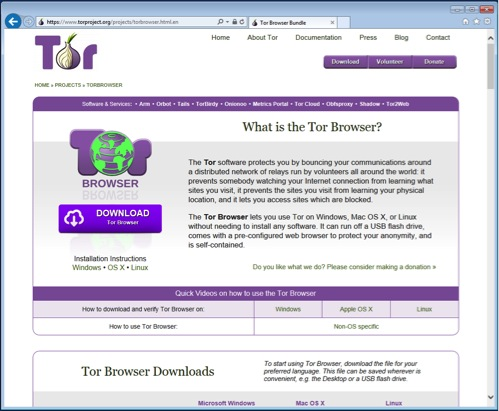
\includegraphics[scale=0.5]{./images/tor2.jpg}
\end{center}
\end{frame}

%----------------------------------------------------------------------------------------
\begin{frame}
\frametitle{Vérifier le Tor Browser téléchargé}
Via les clefs GPG, cf. le tuto sur le site de Tor. \\ \url{https://www.torproject.org/docs/verifying-signatures.html}
\begin{center}
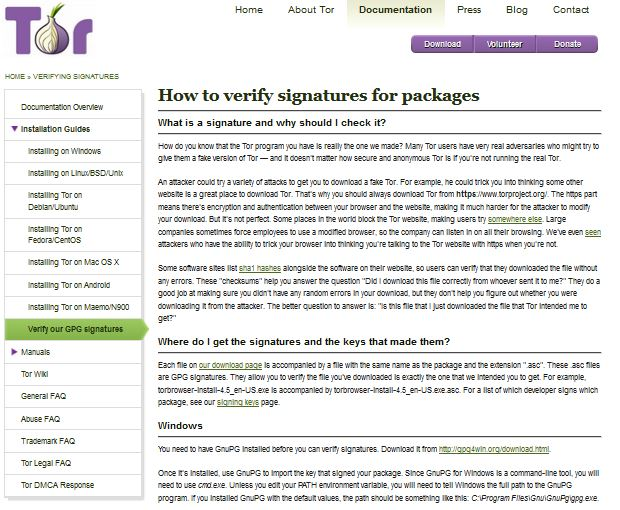
\includegraphics[scale=0.6]{./images/VerifyingSignatures.jpg}
\end{center}
\end{frame}

%----------------------------------------------------------------------------------------
\begin{frame}
\frametitle{Installer le Tor Browser}

\justifying{
Le Tor Browser s'installe comme n'importe quel logiciel Windows, OS X. (voir les tutoriaux si besoin).
\\
Rq : le Tor Browser délenche une alerte avec la suite Symantec (faux positif). 
\\
Pour Ubuntu, GNU/Linux c'est un programme autonome/portable. (On peut aussi l'installer en compilant les sources).
}
\end{frame}

%----------------------------------------------------------------------------------------
\begin{frame}
\frametitle{Lancer le Tor Browser}
\begin{center}
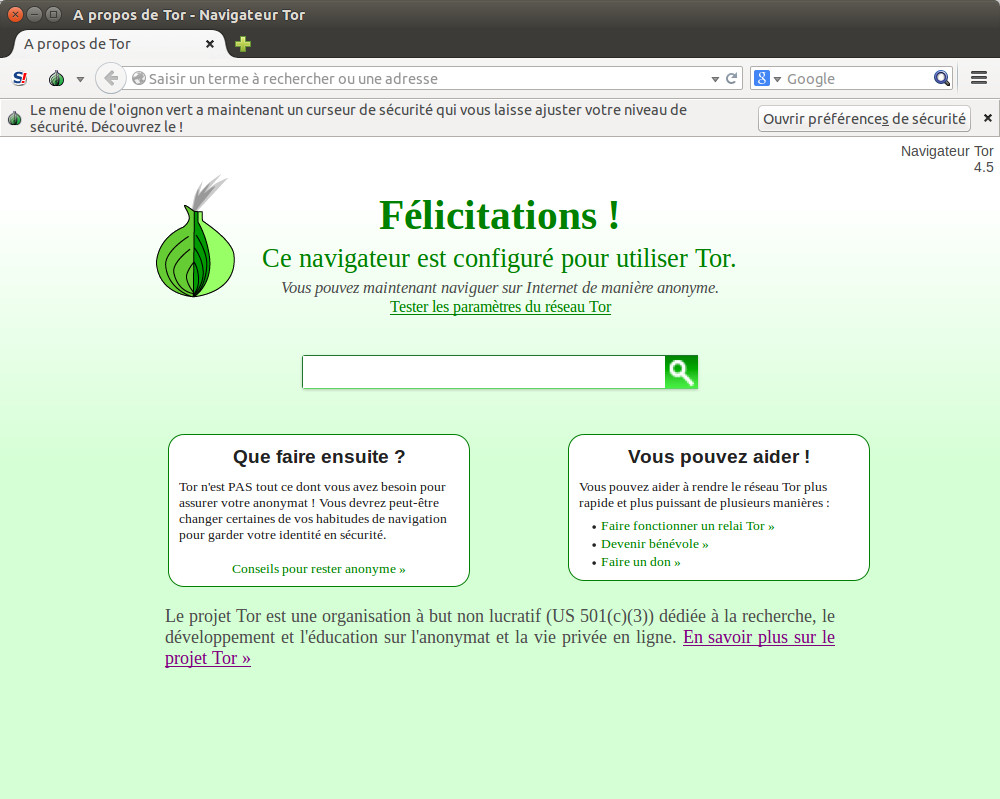
\includegraphics[scale=0.3]{./images/tor_browser03.jpg}
\end{center}
\end{frame}

%----------------------------------------------------------------------------------------
\begin{frame}
\frametitle{Comment être sûr qu'on est bien connecté à Tor?}

\begin{center}
\url{https://check.torproject.org/}
\\~\\
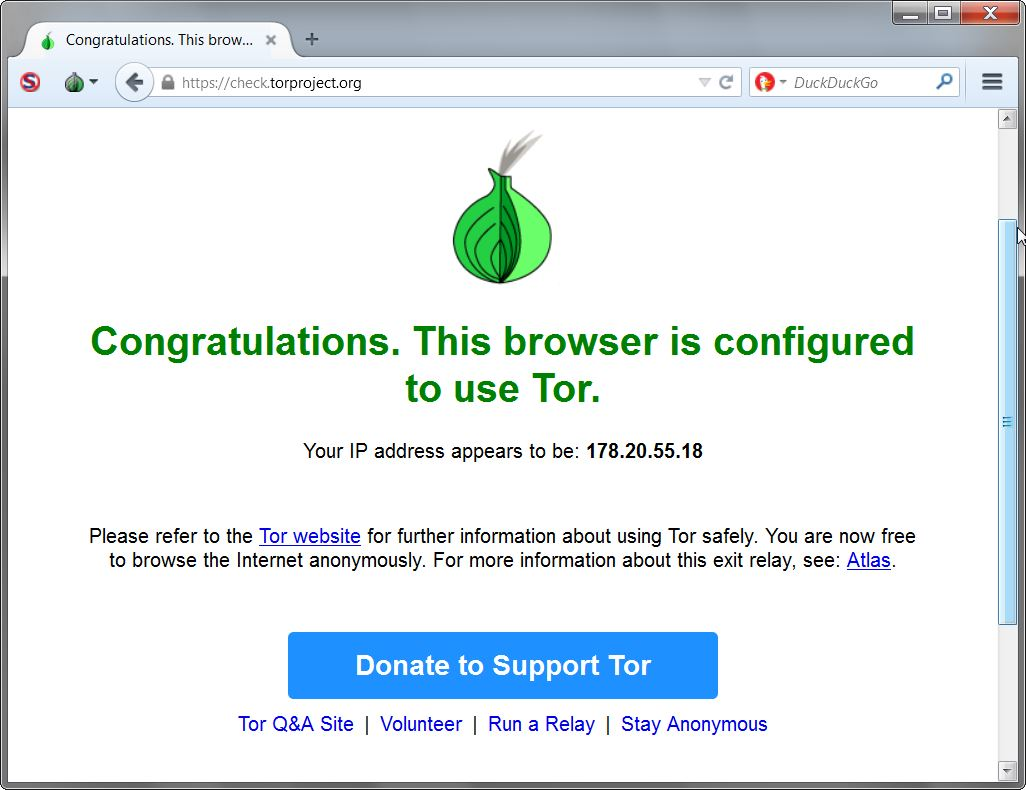
\includegraphics[scale=0.4]{./images/congrats.jpg}
\end{center}
\end{frame}

%----------------------------------------------------------------------------------------
\begin{frame}
\frametitle{Les nouveautés de la version 4.5 1/2}

\begin{center}
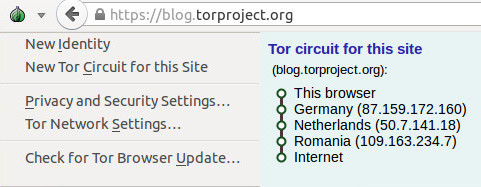
\includegraphics[scale=0.6]{./images/onionmenu.jpg}
\end{center}

\begin{block}{Pour la vie privée}
\begin{itemize}
 \justifying{
\item Visualisation du circuit emprunté (désactivable)
\item Changement de circuit par onglets 
\item Cloisonnement des applications tierces à l'onglet
\item Moteur de recherche par défaut : Disconnect (fournit des résultats de recherche Google)
}
\end{itemize}
\end{block}
\end{frame}

%----------------------------------------------------------------------------------------
\begin{frame}
\frametitle{Les nouveautés de la version 4.5 2/2}
\begin{center}
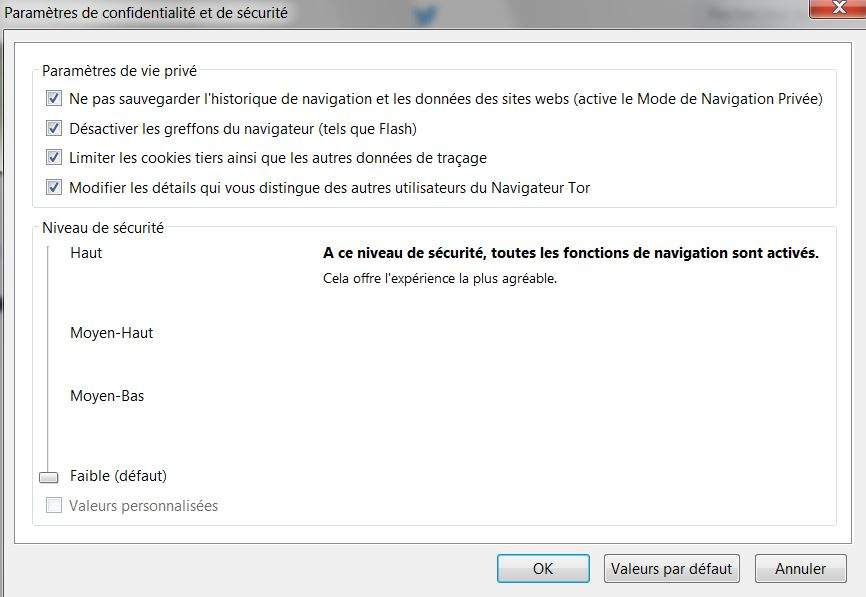
\includegraphics[scale=0.6]{./images/securityslider}
\end{center}
\end{frame}

\begin{frame}
\frametitle{Les nouveautés de la version 4.5 2/2}
\begin{block}{Le curseur de sécurité}
\begin{itemize}
 \justifying{
\item Haut - JavaScript est désactivé sur tous les sites par défaut, certains types d’images sont désactivées.
\item Moyen-Haut - Tous les optimisations de performances JavaScript sont désactivés, certains police fonctionnalités de rendu sont désactivées, JavaScript est désactivé sur tous les non-sites HTTPS par défaut.
\item  Moyen-Bas - HTML5 audio et vidéo sont en mode click-to-play, quelques optimisations de performances JavaScript sont désactivés, les fichiers JAR à distance sont bloqués et quelques méthodes pour afficher des équations mathématiques sont désactivées.
\item  Faible (par défaut) - Toutes les fonctions du navigateur sont activés.
}
\end{itemize}
La compatibilité diminue et la sécurité augmente avec chaque niveau de sécurité.
\end{block}
\end{frame}

%----------------------------------------------------------------------------------------
\begin{frame}
\begin{center}
\Huge{Maintenir le Tor Browser \\ à jour ? }
\\~\\ 
\includegraphics[scale=0.4]{./images/logo_tor.jpg}
\end{center}
\end{frame}

%----------------------------------------------------------------------------------------
\begin{frame}
\frametitle{Vérifier et installer les mises à jour}
\begin{center}
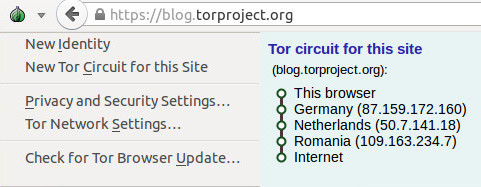
\includegraphics[scale=0.6]{./images/onionmenu.jpg}
\end{center}

\begin{block}{Depuis un TorBrowser}
\begin{itemize}
 \justifying{
\item Cliquer sur "Vérifier les mises à jour"
}
\end{itemize}
La mise à jour se fait via Tor.
\end{block}
\end{frame}

%----------------------------------------------------------------------------------------
\begin{frame}
\frametitle{Tor Browser Launcher}
Pour avoir un Tor Browser toujours à jour, on peut installer le Tor Browser Launcher.
\begin{center}
\url{https://github.com/micahflee/torbrowser-launcher}
\\ 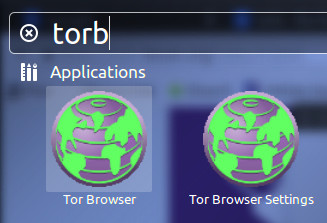
\includegraphics[scale=0.3]{./images/tor_browser01.jpg}
\\ 
\includegraphics[scale=0.3]{./images/tor_browser02.jpg}
\end{center}
\end{frame}
%----------------------------------------------------------------------------------------
\begin{frame}
\frametitle{Tor Browser Launcher}
Il gère : 
\begin{itemize}
\justifying{
\item le téléchargement de la version la plus récente de TBB, dans votre langue et pour votre architecture ;
\item la mise à jour automatique (tout en conservant vos signets et préférences) manuel ;
\item la vérification de la signature GnuPG du TBB (pour être sûr de l’intégrité des fichiers) ;
\item ajoute un lanceur d’application "Tor Browser" dans le menu de votre environnement de bureau.
}
\end{itemize}
\end{frame}
%----------------------------------------------------------------------------------------
\begin{frame}
\begin{center}

\includegraphics[scale=0.3]{./images/tails_logo.jpg}
\\~\\
\url{https://tails.boom.org}
\end{center}
\end{frame}
%----------------------------------------------------------------------------------------
\begin{frame}
\frametitle{Utiliser Tor - Tails}
\justifying{
Tails (The Amnesic Incognito Live System) est un système d'exploitation complet basé sur Linux et Debian, en live.
}
\begin{center}
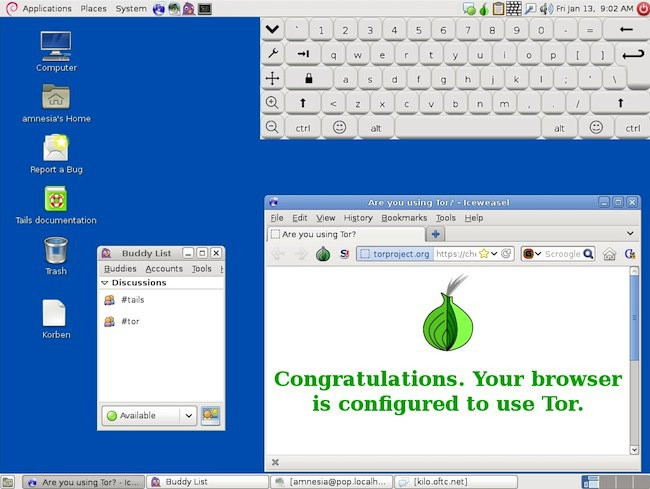
\includegraphics[scale=0.3]{./images/tails.jpg}
\\~\\
\url{https://tails.boom.org}
\end{center}
\end{frame}
%----------------------------------------------------------------------------------------
\begin{frame}
\begin{center}
\Huge{Vous voulez que Tor \\ marche vraiment ?}
\\~\\ 
\includegraphics[scale=0.4]{./images/logo_tor.jpg}
\end{center}
\end{frame}
%----------------------------------------------------------------------------------------
\begin{frame}
\frametitle{Vous voulez que Tor marche vraiment ?}
\justifying{
Vous devrez changer quelques-unes de vos habitudes, et certaines choses ne marcheront pas exactement comme vous le voudrez.
}
\begin{itemize}
\justifying{
\item Ne faîte pas de Torrent via Tor.
\item N'activez pas et n'installez pas de plugins dans le navigateur.
\item Utiliser la version HTTPS des sites webs.
\item Ne consultez pas/n'ouvrez pas de documents téléchargé pendant que vous êtes connecté via Tor.
}
\end{itemize}
\end{frame}
%----------------------------------------------------------------------------------------
\begin{frame}
\begin{center}
\Huge{Soutenir le projet Tor}
\\~\\ 
\includegraphics[scale=0.4]{./images/logo_tor.jpg}
\end{center}
\end{frame}
%---------------------------------------------------------------------------------------
\begin{frame}
\frametitle{Soutenir le projet Tor 1/2}

\begin{block}{NosOignons}
\justifying{
Il existe l'association NosOignons.net, qui propose des nœuds de sortie Tor financés par la communauté.
\url{https://nos-oignons.net}
}
\begin{itemize}
\justifying{
\item En parler
\item Faire un don à NosOignons
}
\end{itemize}
\begin{center}
\includegraphics[scale=0.6]{./images/Dons_nos_oignons.jpg}
\end{center}
\end{block}
 \end{frame}
%---------------------------------------------------------------------------------------
\begin{frame}
\frametitle{Soutenir le projet Tor 2/3}
\begin{block}{Tor Project}
\begin{itemize}
\justifying{
\item Devenir membre de la communauté Tor, Tails
\item Contibuez au code...
\item Faire des tutoriaux, de la traduction...
}
\end{itemize}
\end{block}
 \end{frame}

%---------------------------------------------------------------------------------------
\begin{frame}
\frametitle{Soutenir le projet Tor 3/3}
\begin{center}
\includegraphics[scale=0.25]{./images/jeu_tor.jpg}
\end{center}
\end{frame}

%----------------------------------------------------------------------------------------
\begin{frame}
\begin{center}
\Huge{Questions et discussion}
\end{center}
\end{frame}
%----------------------------------------------------------------------------------------
\end{document}
